% Template for articles
% Based on the ACM SIGPLAN proceedings style
% (c) Farhad Mehta 2020


%%%%%%%%%%-----TEMPLATE
\documentclass[sigplan, nonacm=true, screen=true, timestamp=true, review=false]{acmart}

% Note: Earlier versions acmart before TeXLive 2020 may not support the option `nonacm`
% There is a workaround below for this case.

% The following 4 lines are a workaround in case you are working with a version of acmart that does not support the `noasm` option. 
% \settopmatter{printacmref=false}
% \setcopyright{none}
% \renewcommand\footnotetextcopyrightpermission[1]{}
% \pagestyle{plain}

%%%%%%%%%%-----CONFIGURATION
%%%%%%%%%%-----PACKAGES


%%%%%%%%%%-----COMMANDS
\newcommand{\todo}[1]{TODO: {#1}}


%%%%%%%%%%-----TITLEPAGE
\title{Microservices in a DevOps context}
\subtitle{A review of ``A Systematic Mapping Study on Microservices Architecture in DevOps''}

\author{Christoph Bühler}
\affiliation{University of Applied Science of Eastern Switzerland Rapperswil OST}
\affiliation{MSE Seminar ``Design Science and Empirical Software Engineering''}
\affiliation{Supervisor: Olaf Zimmermann}
\affiliation{Semester: Fall 2020}

\keywords{}

%%%%%%%%%%-----DOCUMENT
\begin{document}

\begin{abstract}
	\textit{
		A systematic mapping study conducts a broad search
		for publications in a research topic and maps the results
		into a condensed form. It gives an overview over the topic,
		the problems and corresponding solutions.
		This paper is a review of such a SMS about the topic of
		``Microservice in a DevOps context''.
		First, the reader is introduced into the various techniques
		and terms used in design science and empirical software
		engineering, then a summary of the reviewed paper is provided
		and then a critical review is stated.
		The study did an excellent job in finding results from the
		academia but the categorical exclusion of gray literature
		lead to missed solutions for given problems.
	}
\end{abstract}


\maketitle

%%%%%%%%%%-----BEGIN_CONTENT

\section{Introduction}

This paper is a review of the systematic mapping study
``A Systematic Mapping Study on Microservices Architecture in DevOps'' \cite{waseem:SMSMSADevOps}.
The goal is to introduce the reader to the topic, explain the used
methods in empirical software engineering, and give a critical review
of the conducted study and the results.

\todo{Describe the used methods to analyze the paper}
\todo{Describe and summarize the result}

The remainder of the paper will introduce terms and principles that are used
in the reviewed study, as well as topics that are needed for the understanding
of the study and this review. Furthermore, a neutral summary of the reviewed study
\cite{waseem:SMSMSADevOps} is provided. After the summary a critical review
is conducted and then a conclusion is derived from the previous sections.


\subsection{Design Science}

Design Science has the main purpose of achieving knowledge and a general understanding
about a domain \cite{hevner:DesignScience}. Design Science contains several guidelines
according to Alan R. Hevner (among other authors). Those guidelines are \cite{hevner:DesignScience}:

\begin{itemize}
    \item \textit{Design as an artefact}: Design Science must produce an artifact
    \item \textit{Problem relevance}: The objective is to develop solutions to relevant business problems
    \item \textit{Design evaluation}: The utility of an artifact must be demonstrated with evaluation methods
    \item \textit{Research contributions}: It must provide clear and verifiable contributions to the topic
    \item \textit{Research rigor}: The research relies on rigorous methods in construction and evaluation of the model
    \item \textit{Design as a search process}: The search for artifacts requires satisfying laws to be in place
    \item \textit{Communication of research}: The targeted audience should be technology-based as well as management based
\end{itemize}


\subsection{Empirical Software Engineering}

Empirical Software Engineering (ESE) provides a solid base for discussion and methods for empirical
research regarding software engineering topics. It has a strong emphasis on \textit{empirical}.

\subsubsection{Systematic Mapping Study (SMS)}

A SMS is a defined method to gather, analyze, classify, and structure a field of interest.
The result of an SMS allows readers and researchers to determine the coverage of the given
field of interest \cite{petersen:SMS}. The analysis focuses on frequency and topics for a
field. It is a defined process in which the following steps take place \cite{petersen:SMS}:

\begin{enumerate}
    \item Define research questions (RQs) and topic
    \item Define search query and parameter
    \item Search for articles and publications in given databases
    \item Analyze and screen the results (i.e., quality assessment and data analysing)
    \item Classify and map the given articles
\end{enumerate}

\subsubsection{Systematic Literature Review (SLR)}

A SLR is a method of ESE to systematically analyze and review a given topic. It uses
methods to collect secondary data and critically reviews the given research study.
The search for additional data can involve published as well as unpublished work
on the subject \cite{siddaway:SLR}.

\subsubsection{Systematic Gray Literature Review (SGLR)}

A SGLR is essentially the same as an SLR with a very important difference:
It does not only consider published and unpublished \textit{peer reviewed} work,
but also ``Gray Literature''. Gray literature is evidence and material that
is not published in commercial and peer reviewed publications \cite{paez:GrayLiterature}.
In the context of computer science, gray literature can provide important statements
and evidence towards topics that are more driven by businesses than by the academia.


\subsection{Microservices and DevOps}

Since the topic of the reviewed paper does conduct an SMS over ``Microservices in DevOps'',
it is utterly important to define those terms so that any reader of this paper
understands the base of the terms on which the conclusions are built upon.

\subsubsection{Microservices}

Microservices (sometimes referred to as ``Microservice Architecture'') is an application
structural style. The style focuses on building several small services that cooperate
together to create an application \cite{richardson:whatIsMSA}. Those services are often deployed on distributed
systems. Most microservices adhere to the following principles \cite{richardson:whatIsMSA}:

\begin{itemize}
    \item Highly maintainable and testable
    \item Loosely coupled
    \item Independently deployable
    \item Organized around business capabilities
    \item Owned by small teams
\end{itemize}

The following image should provide a vague idea of how microservices are structured
and organized \cite{richardson:whatIsMSA}:

\begin{figure}[h]
    \centering
    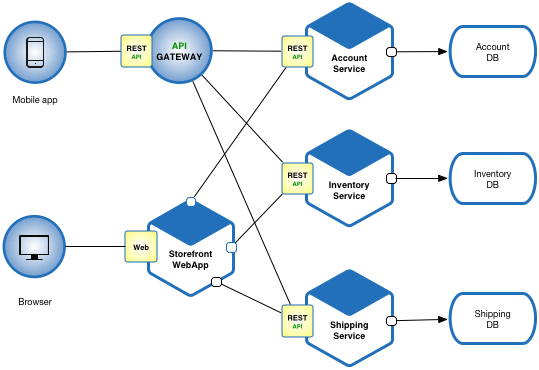
\includegraphics[width=\columnwidth]{images/Microservice_Architecture.png}
    \caption{Example of a Microservice Architecture}
\end{figure}

\subsubsection{DevOps}

The term ``DevOps'' is a mash-up between ``Development'' and ``Operations''. Two
strong and important terms in modern software engineering. The goal of DevOps is to
automate end-to-end in software development and delivery \cite{ebert:DevOps}. It enables
developers to deploy and operate their software autonomously and - in smaller teams - without
any specialized ``Ops'' department. It closes the gap between the classical
software engineers and the operations team which both had their specific tasks. DevOps
provides the means and tools to provide an agile method of software engineering with
\textit{continuous integration} and \textit{continuous deployment} \cite{huettermann:DevOps}.

\section{The reviewed mapping study}
\label{sec:summary}

The general topic of the reviewed paper is to conduct an SMS over the topic
of ``Microservices in DevOps''. We should take into consideration, that the context
is specifically set to ``DevOps''. Recent years and recent developments
raised the attention to the topic significantly. Furthermore, at the
time of writing of the paper, no comprehensive review of the research was
available. The study asks several research questions (RQs) and conducts
a systematic mapping study (SMS) upon two defined search queries. Then,
after screening and analyzing the results, the authors created a mapping
to certain categories and several problems and their solutions.
After a presentation of the results, a wide discussion of the found
results shows some differences between the theory and effective
results \cite{waseem:SMSMSADevOps}.

\subsection{Motivation}

The purpose of the reviewed paper is to create an SMS to understand how 
Microservice Architecture (MSA) is used in conjunction with DevOps.
Furthermore the objective is to identify, analyze and categorize the
existing literature and research around the given topic.
In addition to that, problems and their corresponding solutions - if any - should
be identified. The contribution of the paper to the
academia is a classification of the research, a classification of problems
and their solution, a list of identified research challenges, a classification of
used tools and a list of formal or informal description
tools for MSA \cite{waseem:SMSMSADevOps}.

\subsection{Methodology}

With the goal to not limit the results of such an empirical software engineering method
to one specific research question, the authors conducted an SMS instead of an SLR,
which provides insight and secondary data for a particular question.
The SMS contained three essential steps \cite{waseem:SMSMSADevOps}:

\begin{enumerate}
    \item Planning the mapping study
    \item Collection and analyzing the data
    \item Mapping and documenting the results
\end{enumerate}

The authors built the conducted SMS upon the guidelines purposed by Kai Petersen \cite{petersen:SMS}.

\subsection{Research Questions}

Eight different RQs in four categories were derived 
according to the goal of the paper \cite{waseem:SMSMSADevOps}:

~\\
\begin{table}[H]
    \begin{tabularx}{\columnwidth} { 
        | m{0.12\columnwidth} 
        | X | }
        \hline
        \multicolumn{2}{ | X | }{
            Category 1: Demography, classification,
            and mapping of research
        } \\
        \hline
        RQ1.1
        &
        What is the frequency and type of published research
        on MSA in DevOps? \\
        \hline
        RQ1.2
        &
        What are the existing research themes on MSA in
        DevOps and how can they be classified and mapped? \\
        \hline
        \multicolumn{2}{ | X | }{
            Category 2: Problems, solutions, and challenges
        } \\
        \hline
        RQ2.1
        &
        What problems have been reported when implementing
        MSA in DevOps? \\
        \hline
        RQ2.2
        &
        What solutions have been employed to address the
        problems? \\
        \hline
        RQ2.3
        &
        What challenges have been reported when
        implementing MSA in DevOps? \\
        \hline
        \multicolumn{2}{ | X | }{
            Category 3: MSA description methods, patterns,
            and quality attributes
        } \\
        \hline
        RQ3.1
        &
        What methods are used to describe MSA in DevOps? \\
        \hline
        RQ3.2
        &
        What MSA design patterns are used in DevOps? \\
        \hline
        RQ3.3
        &
        What quality attributes are affected when employing
        MSA in DevOps? \\
        \hline
        \multicolumn{2}{ | X | }{
            Category 4: Tool support and application domains
        } \\
        \hline
        RQ4.1
        &
        What tools are available to support MSA in DevOps? \\
        \hline
        RQ4.2
        &
        What are the application domains that employ MSA in
        DevOps? \\
        \hline
    \end{tabularx}
    \caption{Given research questions}
    \label{tbl:RQs}
\end{table}

The table above (\autoref{tbl:RQs}) shows the research questions that the authors
tried to solve with the systematic mapping study.

\subsection{Search}

To collect data, Waseem et al. used a two-phase-search. The first search was applied
to the selected databases with the created search-query. The secondary
search used a technique called ``snowballing''. ``Forward snowballing''
includes studies that cite the found studies, while ``backward snowballing''
follows the references of the found research material \cite{wohlin:Snowballing}.

The study limited the search to peer-reviewed studies from January 2009 until
July 2018. They chose this particular starting point because the term ``DevOps''
was introduced in the year 2009 \cite{waseem:SMSMSADevOps}.

Since MSA has multiple synonyms and can be in context with DevOps or without
the said context, the following two search-strings were compiled \cite{waseem:SMSMSADevOps}:

\begin{enumerate}
    \item \texttt{((microservi* OR micro-servi*)
    AND (architect* OR design OR structur*) AND DevOps)}
    \item \texttt{(microservice AND DevOps)}
\end{enumerate}

It is worth noting that the contextual part ``DevOps'' is not optional nor is
it a construct like ``microservi*''. This limits the results to publications 
that must contain the term ``DevOps'' in their title.

The search was executed on the following seven databases \cite{waseem:SMSMSADevOps}:

\begin{itemize}
    \item ACM Digital Library (\url{https://dl.acm.org})
    \item IEEE Explore (\url{https://ieeexplore.ieee.org})
    \item Springer Link (\url{https://link.springer.com})
    \item Science Direct (\url{https://www.sciencedirect.com})
    \item Wiley InterScience (\url{https://onlinelibrary.wiley.com})
    \item EI Compendex (\url{https://www.engineeringvillage.com})
    \item ISI Web of Science (\url{https://webofknowledge.com})
\end{itemize}

The execution of the provided search queries on the given databases
yielded a total of 494 studies. After the initial search, the authors
screened and categorized the found studies into relevant and irrelevant
publications. Of the original 494 studies, only 285 were flagged as ``relevant''.
\smsAuthors then analyzed the studies according to six generic screening and one specific
screening aspect. After the screening, 117 remained flagged as relevant.
Those 117 studies were fully read and scored by the authors according to inclusion and
exclusion criteria. At the point when the authors read and assessed all 117 studies,
only 45 studies remained in the relevant category.

In addition to the conducted search, the snowballing technique
yielded additional two studies that were included in the study.
The authors compared the results of the snowball with the found results of the
initial search and then the same practices were applied to those
publications found with the snowball search.

After the search, a total count of 47 different studies remained
relevant for the SMS \cite{waseem:SMSMSADevOps}.

\subsection{Results}

After the conducted search and the thorough analytical readings and classification
of the 47 studies, the collected results were separated in multiple sections
to answer the RQs given in \autoref{tbl:RQs}:

\begin{itemize}
    \item Demography and classification
    \item Problems, solutions and challenges
    \item Description methods, patterns and quality attributes
    \item Tools and application domain
\end{itemize}

The following sections will summarize the found results to
the specific research questions.

\subsubsection{Demography and Classification}

This subsection shall tackle RQ1.1 and RQ1.2 of \autoref{tbl:RQs}.

The conducted search had a year span from 2009 to 2018 \cite{waseem:SMSMSADevOps}.
Despite the broad search parameters of nearly considering a decade worth
of publications, all of the relevant publications were published between
2015 and 2018. The following graph (\autoref{fig:publicationActivity})
should give some insight into the yearly publication rate and the type of publication:

\begin{figure}[H]
    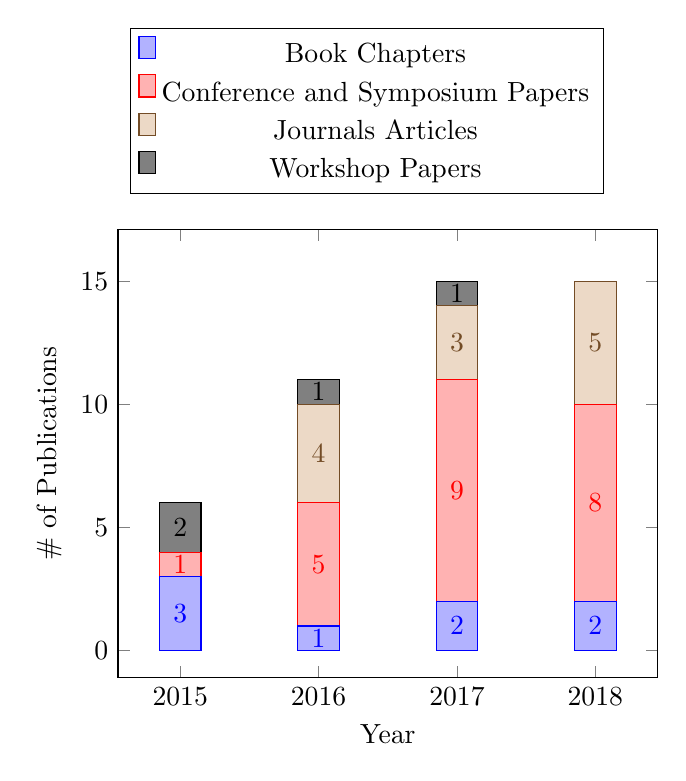
\begin{tikzpicture}
        \begin{axis}[
            ybar stacked,
            bar width=15pt,
            nodes near coords,
            enlargelimits=0.15,
            legend style={
                cells={align=left},
                at={(0.9,1.45)}
            },
            ylabel={\# of Publications},
            xlabel={Year},
            symbolic x coords={2015, 2016, 2017, 2018},
            xtick=data,
            x tick label style={anchor=north},
        ]
            \addplot+[ybar] plot coordinates {
                (2015,3)
                (2016,1)
                (2017,2)
                (2018,2)
            };
            \addplot+[ybar] plot coordinates {
                (2015,1)
                (2016,5)
                (2017,9)
                (2018,8)
            };
            \addplot+[ybar] plot coordinates {
                (2015,0)
                (2016,4)
                (2017,3)
                (2018,5)
            };
            \addplot+[ybar] plot coordinates {
                (2015,2)
                (2016,1)
                (2017,1)
                (2018,0)
            };
            \legend{
                \strut Book Chapters,
                \strut Conference and Symposium Papers,
                \strut Journals Articles,
                \strut Workshop Papers
            }
        \end{axis}
    \end{tikzpicture}
    \caption{Publication activity}
    \label{fig:publicationActivity}
\end{figure}

The distribution of publications over the years gives a detailed intuition
about the general interest of researchers in the specified topic. As seen
in the diagram above, the topic grew more important over the years 2017 and
2018. Since the first publications in 2015 there is an upward trend to
the number of publications \cite{waseem:SMSMSADevOps}.

As for the publication types, over those four years, 23 studies
were published in conference proceedings, twelve in journals, eight in book chapters
and merely four as workshop papers \cite{waseem:SMSMSADevOps}.

The 47 considered papers were all published in 41 venues. The venues
themselves can be divided into four different categories. 17 of the 41
venues count towards the topic \textbf{Internet, Cloud, and Services Computing}.
Another 16 are categorizes as \textbf{Software Engineering} venues. The remaining
eight are split evenly between \textbf{Telecommunications and Networks} with four venues
and \textbf{Multi-Disciplinary computing} also with four venues \cite{waseem:SMSMSADevOps}.

As for RQ1.2, the result shows, that top two subtopics of the publications
are \textit{Approaches} (13 studies) and \textit{Tools} (twelve studies).
The least discussed topic, with only four studies, is \textit{Monitoring}
of microservices \cite{waseem:SMSMSADevOps}.

\subsubsection{Problems, Solutions, and Challenges}

During the SMS, with the aid of a thematic analysis on the
extracted data, a total of 24 problems could be identified.
There exist several problems that could not be mapped with a documented
solution so they represent challenges that need further investigation
to provide the community with possibilities to resolve the problem.

The following lists should give a brief overview of the identified
problems with an associated problem category. Inside the problem domain,
the problems are not specifically ordered \cite{waseem:SMSMSADevOps}.

\textbf{Requirements of MSA-based Systems in DevOps}
\begin{itemize}
    \item Performance Issue due to Lack of Dedicated Access
    to the Host's Hardware
    \item Empowering Developers through Intelligent Software
    \item Performance Overhead due to Fine Grain Decomposition
    \item Scaling MSA-based Systems
\end{itemize}

\textbf{Design of MSA-based Systems in DevOps}
\begin{itemize}
    \item Security and Privacy Across Cloud-Native Applications
    \item Providing Flexible Authentication to Each DevOps Team
    \item Application Decomposition into Microservices
    \item Reducing the Uncertainty in MSA
\end{itemize}

\textbf{Implementation of MSA-based Systems in DevOps}
\begin{itemize}
    \item Managing and Migration Legacy Databases
    \item Modification and Integration of New Functionality in Existing
    Microservices
    \item Operational and Configuration Complexity
\end{itemize}

\textbf{Testing of MSA-based Systems in DevOps}
\begin{itemize}
    \item Testing of MSA-based Systems in DevOps
\end{itemize}

\textbf{Deployment of MSA-based Systems in DevOps}
\begin{itemize}
    \item Frequent Deployment in Different Environments
    \item Complexity in the Dynamic Deployment
    \item Deployment of MSA-based SaaS at Fine Granular Level
    \item Automatic Optimal Deployment of MSA-based Systems
\end{itemize}

\textbf{Monitoring of MSA-based Systems in DevOps}
\begin{itemize}
    \item Logging and Post-Deployment Monitoring
    \item Monitoring and Execution of the Adaptive Actions
    \item Establishing and Maintaining Monitoring Infrastructure
    \item Monitoring Microservices at Run Time
\end{itemize}

\textbf{Organizational Problems}
\begin{itemize}
    \item Introducing DevOps and MSA Culture
    \item People Resistance to Adopting DevOps and Microservices
    \item Less Familiarity with Implementing DevOps
\end{itemize}

\textbf{Resource Management Problems}
\begin{itemize}
    \item Resource management for Development, Deployment,
    and Maintenance of the Cloud-Native Systems
\end{itemize}

For each of the problems in the shown lists, the considered publications
provide at least one solution which can be viewed in ``Figure 6''
of the reviewed study. In general, a purposed idea to tackle multiple
of the problems is to try not to decompose microservice applications
too fine-grain \cite{waseem:SMSMSADevOps}. As for the general problem
category ``designing MSA based systems'', multiple solutions are provided.
Many different architectures are promoted and evaluated \cite{waseem:SMSMSADevOps}.

To implement MSA based systems in a DevOps context, many studies suggest
automated pipelines as well as automatic testing libraries. For communicating
with other services, agnostic (i.e. independent and non-proprietary)
technologies should be used (like REST over HTTP)
to negate the need of knowledge of a specific programming language 
\cite{waseem:SMSMSADevOps}.

Testing MSA based applications and systems should, according to the considered
papers, be tackled with the given testing strategies that are in place
right now. Which means ``unit testing'', ``integration testing'',
``regression testing'', among others \cite{waseem:SMSMSADevOps}.

The topic of deploying MSA based systems is covered mostly by containerization
and tools like ``Docker Compose'' and ``Kubernetes'' \cite{waseem:SMSMSADevOps}.

Monitoring is purposed to be addressed with frameworks like 
``Unicorn''\footnote{\url{https://www.technative.io/unicorn-framework-the-rise-of-devops-as-a-service/}}
and patter-based approaches like Omnia\footnote{Elaborated in \cite{miglerina:Omnia}}.
The general goal should be, that each team that owns the microservice should be enabled
to monitor their responsibilities \cite{waseem:SMSMSADevOps}.

Problems that relate to culture, people, cost, and other organizational
topics are purposed to be dealt with guidelines for adopting to
new structures in organizations. Cross-functional teams should be introduces
and they should receive training to spread the acceptance of the
new technology \cite{waseem:SMSMSADevOps}.

As for the topic of resource management problems, some considered
studies proclaim to use virtualized or containerized approaches
and well established platforms to share the workspace among
the developers \cite{waseem:SMSMSADevOps}.

~\\
On the contrary, three challenges were identified which
remained unresolved by the papers that were accounted for \cite{waseem:SMSMSADevOps}:

\begin{itemize}
    \item Performance issues due to frequent communication
    \item Providing security at runtime
    \item Generating runtime architectural models
\end{itemize}

Performance issues can emerge when using too fine-grain microservices
or when using synchronous communication channels to other services.

Studies found that security tends to be neglected in general which leads 
to severe vulnerabilities at runtime for microservice based architectures.

Generating models for MSA systems at runtime seems to be an unresearched
topic but could be needed to help with decision-making processes in
adaptive system development.


\subsubsection{MSA descriptions methods, patterns, and quality attributes}

The topic of the third category of RQs orbits around descriptive methods
of MSA systems. What methods and patterns are used and which
quality attributes they should suffice. The regarded studies provided
different patterns and methodologies to describe their architectures
and systems. To summarize the found description methods, five categories
emerged \cite{waseem:SMSMSADevOps}:

\begin{enumerate}
    \item Boxes and Lines (without any "framework")
    \item Unified Modeling Language (UML)
    \item Formal method (e.g. $\pi$-Calculus or equivalent)
    \item Architecture Description Language (ADL)
    \item Entity Relationship Diagrams (ERD) or Business
    Process Modeling Notations (BPMN)
\end{enumerate}

Out of the 47 studies, 46 used some kind of description.
The distribution is show in the following diagram:

\begin{figure}[H]
    \begin{tikzpicture}
        \pie [rotate = 180]{
            69.5/Boxes and Lines,
            13/UML,
            8/Formal method,
            6.5/ADL,
            3/Others
        }
    \end{tikzpicture}
    \caption{Distribution of descriptive methods}
\end{figure}

To achieve microservice architecture in complex systems, a multitude of
patterns are purposed over all studies. The SMS identified 38 different design
patterns across all regarded papers. \smsAuthors organized the mentioned
patterns in the following three categories \cite{waseem:SMSMSADevOps}:

\begin{enumerate}
    \item Circuit Breaker (five studies)
    \item ``Migration pattern'' (four studies) \cite{waseem:SMSMSADevOps}
    \footnote{The reviewed SMS does not disclose which specific patterns or languages
    refers to here}
    \item Observer pattern (two studies)
\end{enumerate}

The circuit breaker pattern enables an MSA-based system to ``fail fast''. 
The pattern aims to prevent parts of a microservice architecture to cascade
a failure beyond its own boundaries, which in turn could lead to a total
system failure. Instead of waiting for unresponsive services, after some time
the circuit breaker assumes the worst and deals with the fact that the
work unit has become unavailable \cite{montesi:CircuitBreakers}.

The observer pattern is a software design pattern in which some object (i.e. the ``subject'')
maintains a list of observers. Whenever the subject changes its state, it automatically
notifies all observers \cite{gof:DesignPatterns}.

Regarding affected quality attributes when using MSA in the DevOps context,
the presence of said quality attributes (QA) was confirmed by the SMS.
The QAs were split into two sections, one for positively influenced QAs when
using microservices and one for the negative influenced ones \cite{waseem:SMSMSADevOps}.

\textbf{Positive}
The studies listed the following QAs as being positively influenced:
\begin{itemize}
    \item Deployability (42 studies)
    \item Scalability (32 studies)
    \item Performance (26 studies)
    \item Maintainability (27 studies)
    \item Monitoring (23 studies)
    \item Testability (22 studies)
    \item Flexibility (20 studies)
    \item Availability (19 studies)
    \item Efficiency (19 studies)
    \item Security (ten studies)
    \item Portability (six studies)
    \item Compatibility (five studies)
    \item Modifiability (five studies)
    \item Usability (one study)
\end{itemize}

\textbf{Negative}
Some studies listed the following QAs as being negatively influenced:
\begin{itemize}
    \item Security (eleven studies)
    \item Performance (nine studies)
    \item Scalability (two studies)
    \item Reliability (two studies)
    \item Availability (one study)
    \item Compatibility (one study)
    \item Maintainability (one study)
    \item Modifiability (one study)
    \item Usability (one study)
\end{itemize}

To have a view from positively mentioned against negatively mentioned,
consider the following chart:

\begin{figure}[H]
    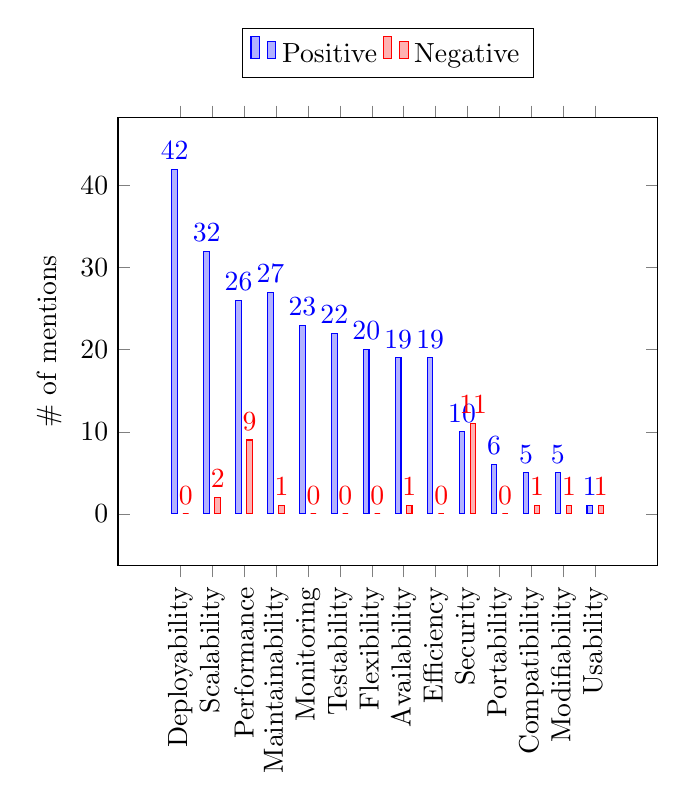
\begin{tikzpicture}
        \begin{axis}[
            ybar,
            bar width=2pt,
            enlargelimits=0.15,
            legend style={
                at={(0.5,1.2)},
                anchor=north,legend columns=-1
            },
            ylabel={\# of mentions},
            symbolic x coords={
                Deployability,
                Scalability,
                Performance,
                Maintainability,
                Monitoring,
                Testability,
                Flexibility,
                Availability,
                Efficiency,
                Security,
                Portability,
                Compatibility,
                Modifiability,
                Usability
            },
            xtick=data,
            x tick label style={rotate=90,anchor=east},
            nodes near coords,
            nodes near coords align={vertical},
        ]
            \addplot coordinates {
                (Deployability,42)
                (Scalability,32)
                (Performance,26)
                (Maintainability,27)
                (Monitoring,23)
                (Testability,22)
                (Flexibility,20)
                (Availability,19)
                (Efficiency,19)
                (Security,10)
                (Portability,6)
                (Compatibility,5)
                (Modifiability,5)
                (Usability,1)
            };
            \addplot coordinates {
                (Deployability,0)
                (Scalability,2)
                (Performance,9)
                (Maintainability,1)
                (Monitoring,0)
                (Testability,0)
                (Flexibility,0)
                (Availability,1)
                (Efficiency,0)
                (Security,11)
                (Portability,0)
                (Compatibility,1)
                (Modifiability,1)
                (Usability,1)
            };
            \legend{
                \strut Positive,
                \strut Negative
            }
        \end{axis}
    \end{tikzpicture}
    \caption{Influenced Quality Attributes}
\end{figure}

\subsubsection{Tool support and application domains}

The fourth category of research questions regards tooling support
and given application domains. The SMS identified 50 different tools and
11 application domains.

The various tools can be seen in Fig. 7 in the SMS \cite{waseem:SMSMSADevOps}.
The authors categorized them in the following list:

\begin{itemize}
    \item Security Services and Tools (14 tools)
    \item Monitoring Tools (eleven tools)
    \item Continuous Integration Tools (seven tools)
    \item Testing Tools (six tools)
    \item Configuration Management Tools (five tools)
    \item Build Tools (five tools)
    \item Version Control Tools (two tools)
\end{itemize}

The last RQ that is to be answered, is which application domains
exploit the combination of MSA with DevOps. The SMS pinpointed nine
application domains with analyzation of the systems and topics
in the regarded studies. \smsAuthors identified the following
application domains in their study \cite{waseem:SMSMSADevOps}:

\begin{itemize}
    \item Not Mentioned (15 studies) \footnote{Those 15 studies
    did not mention any specific information regarding application
    domains}
    \item Software Development Tools and Framework (eleven studies)
    \item Telecommunication (six studies)
    \item Mobile Software (four studies)
    \item E-Commerce system (three studies)
    \item Embedded system (three studies)
    \item Financial software (three studies)
    \item Healthcare software (one study)
    \item Webserver (one study)
    \item Distributed system (one study)
    \item Autonomic Management System (one study)
    \item Betting and Gaming (one study)
    \item Web Blog (one study)
    \item eServices Developments (one study)
    \item Container Management System (one study)
    \item Content Management (one study)
    \item Software for non-profit (one study)
\end{itemize}

As this list shows, beside studies that did not mention their concrete
application domain, ``Software Development Tools and Framework''
has gained the most attention of all identified application domains
in the study \cite{waseem:SMSMSADevOps}.

\subsection{Discussion}

The following sections summarizes the ``Discussion'' of the SMS. The study
analyzed the found results and explained certain trends.

\subsubsection{Research status and themes}

The limitation of the search to peer-reviewed literature from January 2009 to
July 2018 is based on the ``creation'' of the terms MSA and DevOps.
But the rise of papers and studies followed seven years later, around January 2016.
The study noticed, that 41 papers were published from January 2016 until July 2018
\cite{waseem:SMSMSADevOps}.

As seen in the systematic classification of the research themes, the most recurring
topics are ``Tools'' with 13 studies, ``Approaches'' with twelve studies and
``Development and Deployment'' with twelve studies. This indicates, that the research
is not only centered around new tools, but also regards development life-cycles
as well. On the other hand, there were no publications found that focus on
the topic of ``Requirements Engineering'', be it practices or any other
activities \cite{waseem:SMSMSADevOps}.

\subsubsection{Problems and solutions}

The given solutions in the regarded publications consist, of
design patterns, guidelines, frameworks, etc. For example,
Domain Driven Design (DDD) and Model View Controller (MVC) patterns
are recommended for decomposing an application into a microservice oriented
system. The SMS also states that there are no studies found that
address testing strategies for MSA based systems. As for optimal deployment
of MSA, a very popular solution is the usage of containerization and Kubernetes
\cite{waseem:SMSMSADevOps}.

\subsubsection{Challenges}

A big concern in several papers is performance of such MSA based systems.
The impact can be due to frequent communication between microservices.
Also, poorly engineered architectures can lead to wide spreaded requests
across the whole system. Also, when containers are used, the hardware underneath
has a high impact on performance. The study shows that Amazon EC2 containers are
worse than applications deployed on Amazon EC2 VMs \cite{waseem:SMSMSADevOps}.

The second topic that gets addressed with high frequency, is security. When just ``translating''
applications to MSA, most of the time, security concerns arise. MSA based systems
create complex access control scenarios without any matured patterns to harden
the systems against attackers \cite{waseem:SMSMSADevOps}.

\subsubsection{Description methods and MSA design patterns}

Most studies use just plain, informal boxes and lines as well as UML to
describe microservice architectures. Other methods, like formal $\pi$-Calculator
among others, are used rarely. The SMS argues, that this could be adressed with
the creation of a standard description method for describing MSA
\cite{waseem:SMSMSADevOps}.

The used design patterns are shown in the corresponding table in the SMS.
The most observed pattern is the ``Circuit Breaker'' \cite{montesi:CircuitBreakers} pattern which indicates,
that cascading failures are a major concern. Next in line is the ``Migration
Pattern'' \cite{waseem:SMSMSADevOps} that recommends various best practices for the transition from
a monolytic application to a MSA based system.
A not so well covered topic are patterns and recommendations
that support CI/CD in MSA \cite{waseem:SMSMSADevOps}.

\subsubsection{Application domains}

The SMS observed, that a third of the studies did not provide a specific application
domain, nor any information to which domain they may count. The rest of the publications
could be categorized into different application domains. The most referenced domain
is ``Software Development Tools and Framework''. This results indicate, that MSA
in the DevOps context is not bound to a specific application domain but rather is
an improvement to a broad range of application domains such as healthcare, finance sector
and embedded systems \cite{waseem:SMSMSADevOps}.

\section{Critical review of the paper}
\label{sec:review}

The following section is a critical review of the conducted study.
The review contains statements about the used empirical engineering methods
as well as the found results and the followed discussion about the results.

As a general critique, the layout of the study should help
the reader through the paper smoothly.
There are many tables and figures which explain the results
quite efficient and to the point, but the layout of the study forces the
reader to jump around when going through it. It could have been
a better approach to move all figures and tables to an appendix
and have the text reference them.

\subsection{Definitions}

Some abbreviation (like ``SLR'') are introduced in the later stage of
the study and leave the reader without knowledge about their meaning
in the first few sections.

The general definition of microservice architecture (MSA) and DevOps
are accurate to the literature and are well described. There are
many references which allow the reader to further read into the topic
of MSA and DevOps.

\subsection{Empirical Research Methods}

The study used the purposed guidelines of peer-reviewed publications
to conduct the SMS. The authors did adjust and combine some of the guidelines
according to the peculiarities of the topic.

\subsubsection{Research Questions}

The research questions are well structured into categories.
However, the RQs in categories two to four appear too broad
in my opinion. Some of the questions should be split up into finer definitions or
should be more specific.

\textbf{RQ2.1} \textit{``What problems have been reported 
when implementing MSA in DevOps?''} \wsl:
The problems that have been reported should be split
into categories. Are the problems centered around general understanding of
MSA, is it troubling to deploy and maintain a MSA based system or
is the development (migration or new solution) process problematic?

\textbf{RQ3.2} \textit{``What MSA design patterns are used in DevOps?''} \wsl:
The stated question about design patterns does
cover \textit{all possible pattern-topics}. So the question addresses
patterns that are used for developing microservice applications and
other patterns that recommend a way to migrate a monolith to a MSA.
A categorization between the patterns would help the reader to
grasp the results in the correct context. As an example this could be done
with a \textit{4+1 viewpoint} model (\textit{Logical view},
\textit{Development view}, \textit{Process view}, \textit{Physical view},
and \textit{Scenarios}) from P.B. Kruchten \cite{kruchten:Viewmodels}.

\textbf{RQ4.1} \textit{``What tools are available to support MSA in DevOps?''} \wsl:
A similar categorization should be used for the
research question about available tooling. Currently, this question
ranges from planning tools (e.g. Jira) to tools for version control
(e.g. GitHub).

\subsubsection{Search strategy and Snowballing}

The search for publications is conducted thoroughly. Many results
are found which is a good sign for the search itself. It is an excellent
idea to use two search queries to search for ``microservices'' and
``architecture'' in conjunction with the DevOps context.

On the topic of the search boundaries, it can be said that ``January 2009''
does include all the results that are found. Since the term ``microservice''
was defined by Martin Fowler in 2014 \cite{fowler:microservices} the lower
bound of the search could be set to ``January 2014''. According to Fowler,
the term ``MSA'' was not precisely defined until then.
The upper bound on the other hand is set to ``July 2018'' which is most likely
the date when the search was executed. While the SMS does explain
why January 2009 was selected as the lower bound, it is not stated
at all why July 2018 is the upper bound. The reviewed study was published
in the year 2020, but since the searched publications were limited
to the year 2018, many new techniques and publications were ignored.

The limitation of the search to only allow peer-reviewed publications
to be relevant does filter out some solutions to given problems and
even challenges. In computer science, one big driving force
of innovation are companies that need solutions and tools for the
current problems at hand. Companies tend to have shorter innovation-cycles
than the academia. With this matter in mind, many solutions are only described
in blog posts or as showcases. It would have been a good approach to search for the problems along
the peer-reviewed papers and allow some gray literature in the
discussion to give advice to certain challenges and/or problems.

The search queries
``\texttt{((microservi* OR micro-servi*) AND (architect* OR design OR structur*) AND DevOps)}''
and ``\texttt{(microservice AND DevOps)}'' \wsls
also exclude a relatively large portion of potential publications since 
the term ``DevOps'' is mandatory and without variants. While different
writing styles and variants were used for the term ``Microservice'', the term ``DevOps''
is just plainly searched. There could also be material, that does not
contain the term in the title at all. Those papers are excluded as well.

\subsubsection{Quality assessment}

The given screening criteria are well defined and create
an exact baseline for the found papers such as the
language of the publication or if it is peer-reviewed.

The stated qualitative criteria are nicely balanced
and provide a good assessment of the found publications.
It does make sense to search for clearly stated motivations,
problems, and solutions in the found studies. Furthermore, it is
eminent to know the limitations of the studies. The increased
weight of the specific criteria versus the generic ones does
help to search for the targeted publications that are relevant
for the topic of the SMS.

\subsection{Results and Discussion}

\smsAuthors extensively describe the derived results and
the subsequent discussion. Some findings and argumentation
spark questions however.

\subsubsection{Problems and Solutions}

One of the stated problems in the SMS is that it did not find
any studies about testing of MSA based systems in DevOps \cite{waseem:SMSMSADevOps}.
Since gray literature was excluded from the search, some relevant
publications from the industry were ignored. In the specific topic
of testing MSA based and cloud-ready systems, Netflix provided
a detailed description about an approach in their
blog\footnote{\url{https://netflixtechblog.com/}}.

Among other established testing techniques (Unit testing, Integration testing, etc.)
Netflix uses something they call ``Chaos testing''. The goal of this
so called ``Chaos Monkey''\footnote{\url{https://github.com/Netflix/chaosmonkey}}
is to test whole systems for resiliency by shutting down services,
nodes, and entire clusters at random times. This is a specific testing use-case
for MSA and cloud-ready systems. Since no system can guarantee 100\% up-time,
the chaos monkey introduces interruptions that the system must handle.
The system should depend on some services not being available. With that
in mind, a resilient system can be created \cite{netflix:SimianArmy,basiri:ChaosEngineering}.

\subsubsection{Research Challenges}

The first research challenge \textit{Performance issues
due to frequent communication} does state that too fine-grain
MSA introduce complexity. I would like to argue, that nearly
all fine-grain systems introduce complexity. The biggest issue, in terms of performance,
with fine-grain MSA is the direction of the call-flow.
Each level in this ``service depth'' does add to the total amount of
time needed to compute the request of the user.

\begin{figure}[ht]
    \centering
    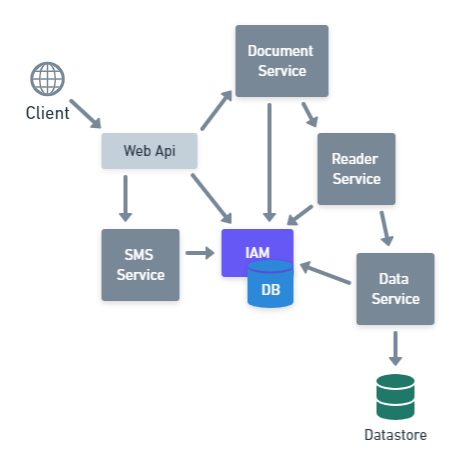
\includegraphics[width=\columnwidth]{images/service_depth.png}
    \caption{Deep MSA problem}
    \label{fig:deepMSA}
\end{figure}

The problem with ``service depth'' is not the performance
impact of computation itself in a work unit, but the general impact
on the overall system when chaining subsequent units together.
\autoref{fig:deepMSA} shows such a scenario. For the sake of
simplicity, let us assume that each call in \autoref{fig:deepMSA}
(i.e. Client to Api, Api to IAM\footnote{\label{fn:IAM}Identity and Access Management},
Service to Service, and Service to Datastore) takes \texttt{100ms}.

The assumed time contains computation, transformation from and to
the transport protocol and the round trip.
The basic idea is to show the performance impact when chaining services
into a ``deep system''.
With the given description, let us consider the following two scenarios:

\begin{enumerate}
    \item \textit{Client sends a SMS}:
    Client $\rightarrow$ Api $\rightarrow$ SMS Service. Api and SMS Service make
    a credentials check at the IAM\textsuperscript{\ref{fn:IAM}}.
    The successful response to the client
    is delivered after: $4 * 100ms = 400ms$
    \item \textit{Client requests a document}:
    Client $\rightarrow$ Api $\rightarrow$ Document Service $\rightarrow$
    Reader Service $\rightarrow$ Data Service $\rightarrow$ Data Store.
    All services check the credentials with the IAM\textsuperscript{\ref{fn:IAM}}.
    The successful response to the client
    is delivered after: $100ms \text{(Client)} + 4*100ms \text{(IAM)}
    + 3*100ms \text{(Services)} + 100ms \text{(DB)} = 900ms$
\end{enumerate}

A possible solution to this particular problem is to plan
the microservices and the corresponding architecture accordingly.
Frequent review of the current architecture and refactoring \cite{zio:ARforCloud}
if needed are key to prevent too deep services. This can happen
in a very agile way since one of the basic goals of MSA is
to have fast deployable artifacts.

The usage of synchronous HTTP calls will definitely result
in a performance penalty. Systems like ``Google PubSub'' could help
mitigate this bottleneck and create the possibility to scale
instances of microservices on the horizontal scale.
Furthermore, Kubernetes, among other orchestration platforms, provide developers with
battle-proof tools to scale services with load-balancing features
such as ``services'' which map to instances of the given services.

The statement about hardware is accurate. Depending on the hardware,
the performance of the whole MSA based system will vary. For example,
let us consider a microservice that was developed with
PHP\footnote{\url{https://www.php.net/}}. Depending on the used framework,
PHP loads the \texttt{*.php} script files for each and every call that
is made to the application. Since those script files are not cached
in memory or any compiled form, when the underlying hardware contains
storage with normal hard disk drives instead of solid state disks,
the performance impact is huge. On the other hand, a compiled application
like a C\# Web-Application does load itself into the memory of the
container and does not have the need to load some files for each request.

The second challenge \textit{Providing security at runtime} does
describe some of the current problems. Security is a hard topic
on itself and in conjunction with MSA, it does not get any easier.
Several patterns exist, that can provide some mechanism of security,
but as always, there is no silver bullet. A good strategy to
authenticate and authorize calls made from a source would be the usage
of OpenID Connect (OIDC) \cite{Siriwardena:OIDC}. OIDC enables
a system to have a centralized user and access management. The
calls are authenticated with a token and each microservice can check
if the call is authenticated and valid or not. As for authorization,
the central identity server can provide endpoints to fetch roles
or other means of authorization logic to check if the call is allowed
in the given microservice with the provided token.

\subsubsection{Quality attributes}

The SMS does a good job at showing the positive and negative
statements of the relevant studies. The comparison and categorization
is well done and gives an overview which topics contain solutions
for non-MSA-problems and which problems are newly introduced by
MSA and DevOps itself. The most important statement here is the security
concern. Security is and will be a part of any public application
and therefore is a central topic.

\subsubsection{Tool support}

The validity of this part of the results is questionable.
The listed and found tools over all the regarded publications mix
use-cases of various tools. As an example, ``Jira'' is listed
as monitoring tool, but I would argue, that ``Jira'' is definitely
not a tool for monitoring, regardless of the topic or the context.
The results show the provide tools in the stated topics, but the
discussion could have critically analyzed the tools and their positions
in the categories. Another example is ``Filebeat'', which is listed under
``Security Services and Tools''. But Filebeat should be listed under
monitoring or logging tools since it reads files produced by a service
and sends them to an ELK\footnote{\url{https://www.elastic.co/elastic-stack}} stack.
Filebeat itself does nothing in terms of security, it is a log analyzer.

Furthermore, the vast majority of the listed tools are ``Enterprise Tools''.
This does not necessarily mean they are not worth a try,
but they tend to be aged and not created according to the
newest and latest patterns and practices.

There are many open-source industry driven tools missing. Many
modern companies use newer and more state-of-the-art tools.
A few examples:

\begin{itemize}
    \item \textbf{Clair} \textit{Security}:
    A security scanner for containerized software that can statically analyze
    built containers for issues
    (\url{https://blogs.vmware.com/opensource/2019/10/31/clair-container-security/})
    \item \textbf{Jaeger} \textit{Monitoring}:
    Open-Source tracing tool that enables the developers to trace calls
    trough a complex system from end to end
    (\url{https://www.jaegertracing.io/})
    \item \textbf{GitHub Actions} \textit{CI}: The automated continuous integration
    platform from github
    \item \textbf{Gitlab CI} \textit{CI}: The automated continuous intregration
    platform from gitlab
    \item \textbf{ArgoCD} \textit{Configuration Management}: ArgoCD is an
    application that manages applications declaratively (GitOps pattern).
    Instead of using a CI pipeline to deploy an application to a cluster,
    the CI pipeline only creates the artifact (e.g. a Docker image) and publishes
    it somewhere. Then the pipeline can update the declarative description
    of the application with the new version of the image and Argo will
    be aware of the change and therefore will deploy the new image
    (\url{https://argoproj.github.io/argo-cd/})
\end{itemize}

The industry has produced many more tools that solve some of the stated
problems during the past years. Most of them were only mentioned or described
in gray literature.

\section{Conclusion}

With this paper, we created a critical review
of the systematic mapping study
``A Systematic Mapping Study on Microservices Architecture in DevOps''
by \smsAuthors \wsl.

In \Autoref{sec:introduction} the reader was introduced into the
topic and various prerequisites were specified. We introduced
terms like ``Microservice'', ``DevOps'' and methodologies from
design science and empirical software engineering like ``SMS'',
``SLR'', and ``SGLR''.

Within \Autoref{sec:summary} the paper gave a brief objective
summary for the reviewed SMS. The methods used are described
with the conducted search and the found results. Afterwards
the reader got an overview of the held discussion in the paper
and the derived research challenges.

The critical review in \Autoref{sec:review} then gives the
reader a subjective review with critics to certain topics.
In general the study covers a broad area of research
and did sum up its results in a clean way.

The reviewed SMS yielded good results in the specific
context of ``DevOps''. However the search terms that were
used did limit the results to publications what contain the
word ``DevOps'' in their title. This excluded results which
may have opinions and solutions to found problems.
Furthermore, the categorical exclusion of gray literature
did limit the result to problems, solutions and tools from the
academia without the results of the industry. The industry is a key driver
for this topic in computer science and should be
included in such a study. One possible outcome could have been
that more research should be conducted based on statements and
findings from the industry.

As a result of this review, a conclusion could be to conduct
another study with regard to the problems stated in \wsls and
map solutions from gray literature to their problems. Another
possibility is to create further research to topics
presented as possible solutions in \Autoref{sec:review} and
create peer-reviewed publications that include gray literature.


%%%%%%%%%%-----BIBLIOGRAPHY

%% \nocite{latexDerivationTree}

\bibliographystyle{alpha}
\bibliography{bibliography}

%%%%%%%%%%-----END_DOCUMENT

\end{document}
